% ===========================================================================
% WinLIC: A Windows-Compatible Offline Multi-Modal Gaussian Splatting
%          Framework with Pluggable Sensor Integration
%
% Compile: pdflatex main && bibtex main && pdflatex main && pdflatex main
% ===========================================================================
\documentclass[11pt, a4paper]{article}

%% ---- Math & graphics ----
\usepackage{amsmath, amsfonts, amssymb}
\usepackage{mathtools}
\usepackage{booktabs}
\usepackage{graphicx}
\usepackage{geometry}
\geometry{margin=2.5cm}

%% ---- TikZ ----
\usepackage{tikz}
\usetikzlibrary{positioning, arrows.meta, calc, fit, shapes.geometric,
                backgrounds, decorations.pathreplacing, patterns, shadows}

%% ---- Algorithms ----
\usepackage{algorithm}
\usepackage{algpseudocode}

%% ---- Listings ----
\usepackage{listings}
\usepackage{xcolor}

%% ---- Hyperlinks ----
\usepackage{hyperref}
\hypersetup{colorlinks=true, linkcolor=blue!70!black, citecolor=green!50!black, urlcolor=blue!80!black}

%% ---- xspace (must load before commands that use \xspace) ----
\usepackage{xspace}

%% ---- Custom commands ----
\newcommand{\SEthree}{\mathrm{SE}(3)}
\newcommand{\SOthree}{\mathrm{SO}(3)}
\newcommand{\GaussianMap}{\mathcal{G}}
\newcommand{\PointCloud}{\mathcal{P}}
\newcommand{\DepthMap}{\mathbf{D}}
\newcommand{\Image}{\mathbf{I}}
\newcommand{\Tcw}{T_{C\leftarrow W}}
\newcommand{\Twc}{T_{W\leftarrow C}}
\newcommand{\Rcw}{R_{C\leftarrow W}}
\newcommand{\tcw}{\mathbf{t}_{C\leftarrow W}}
\newcommand{\winlic}{\textsc{WinLIC}\xspace}
\newcommand{\gaussianlic}{\textsc{Gaussian-LIC2}\xspace}

%% ---- TikZ styles ----
\tikzset{
  block/.style={rectangle, draw, rounded corners, minimum height=0.9cm,
                minimum width=2.2cm, align=center, font=\small,
                fill=blue!8, drop shadow={shadow xshift=1pt, shadow yshift=-1pt}},
  blockgreen/.style={rectangle, draw, rounded corners, minimum height=0.9cm,
                     minimum width=2.2cm, align=center, font=\small,
                     fill=green!10, drop shadow={shadow xshift=1pt, shadow yshift=-1pt}},
  blockorange/.style={rectangle, draw, rounded corners, minimum height=0.9cm,
                      minimum width=2.2cm, align=center, font=\small,
                      fill=orange!12, drop shadow={shadow xshift=1pt, shadow yshift=-1pt}},
  blockred/.style={rectangle, draw, rounded corners, minimum height=0.9cm,
                   minimum width=2.2cm, align=center, font=\small,
                   fill=red!8, drop shadow={shadow xshift=1pt, shadow yshift=-1pt}},
  sensor/.style={cylinder, shape border rotate=90, draw, minimum height=0.8cm,
                 minimum width=1.5cm, align=center, font=\footnotesize,
                 fill=yellow!15},
  arrow/.style={-{Stealth[length=2.5mm]}, thick},
  dasharrow/.style={-{Stealth[length=2.5mm]}, thick, dashed},
  group/.style={rectangle, draw, dashed, rounded corners, inner sep=8pt,
                label={[font=\footnotesize\bfseries]above:#1}},
}

\title{\winlic: A Windows-Compatible Offline Multi-Modal \\
       Gaussian Splatting Framework with Pluggable Sensor Integration}

\author{Arthur Li Rui}
\date{October 2026}

\begin{document}
\maketitle

\begin{abstract}
We present \winlic, a standalone, operating-system-agnostic offline reconstruction
framework that fuses multi-modal sensory data---LiDAR point clouds, indirect
time-of-flight (iToF) depth streams, stereo vision, and inertial measurements---to
produce high-quality initialization point clouds and colour observations for
3D Gaussian Splatting (3DGS) scene reconstruction.
Unlike prior real-time Gaussian SLAM systems that are tightly coupled to the
Robot Operating System (ROS) and restricted to Linux, \winlic eliminates all
ROS dependencies, introducing a pluggable sensor source abstraction layer that
accommodates both offline file-based datasets and live camera streams (e.g.,
Orbbec Femto Mega) through a uniform \texttt{ISensorSource} interface.
The framework preserves the core Gaussian Splatting mapping algorithm of
\gaussianlic while decoupling it from the real-time front-end, enabling
batch-mode processing on commodity Windows workstations.
We describe the system architecture, multi-modal depth fusion strategy,
and the design of the extensible sensor integration layer, accompanied by
detailed pipeline diagrams.
\end{abstract}

\tableofcontents
\newpage

% ---- Sections ----
% ===========================================================================
% Section: Introduction
% ===========================================================================
\section{Introduction}
\label{sec:introduction}

3D Gaussian Splatting (3DGS)~\cite{kerbl2023_3dgs} has emerged as a powerful
primitive for photo-realistic scene representation, achieving real-time
rendering quality that surpasses NeRF-based methods while maintaining
explicit, editable geometry. The integration of 3DGS with simultaneous
localization and mapping (SLAM) pipelines---particularly those fusing
LiDAR, inertial, and camera data---has produced systems such as
\gaussianlic~\cite{lang2026_gaussianlic2} that achieve real-time,
photo-realistic mapping on a single moving platform.

However, existing Gaussian SLAM systems share a critical limitation: they are
\emph{tightly coupled to the Robot Operating System} (ROS) and therefore
restricted to Linux environments. The ROS dependency manifests at multiple
levels: message-passing via \texttt{roscpp}, image transport via
\texttt{cv\_bridge}, point cloud conversion via \texttt{pcl\_conversions},
pose messages via \texttt{geometry\_msgs}, and coordinate transforms via
\texttt{tf}. This coupling prevents deployment on Windows workstations,
limits interoperability with commercial sensor SDKs (e.g., Orbbec,
Intel RealSense), and complicates integration into industrial pipelines
that operate outside the ROS ecosystem.

Furthermore, the real-time design of these systems assumes a continuous
online data stream, making them suboptimal for \emph{offline} batch
processing of pre-recorded datasets---a common workflow in surveying,
inspection, and content production.

We address these limitations with \winlic, a framework that makes the
following contributions:

\begin{enumerate}
    \item \textbf{ROS-free architecture.} We refactor the Gaussian-LIC2
    mapping pipeline to eliminate all ROS dependencies, producing a
    standalone C++ application that builds with pure CMake and runs on
    both Windows (MSVC) and Linux (GCC).

    \item \textbf{Pluggable sensor interface.} We design an abstract
    \texttt{ISensorSource} interface that decouples the reconstruction
    pipeline from the data source. Offline file-based readers and live
    camera SDKs (Orbbec, future sensors) are integrated through a uniform
    four-method interface.

    \item \textbf{Multi-modal depth fusion.} We introduce a
    confidence-weighted depth fusion module that combines sparse LiDAR
    depth, dense iToF depth, and stereo SGM depth into a single
    high-quality depth map, which is then completed by a TensorRT-based
    neural network (SPNet).

    \item \textbf{Preserved algorithm fidelity.} The core Gaussian
    Splatting algorithm---initialization, map extension, optimization,
    and densification---is preserved verbatim from \gaussianlic, ensuring
    reconstruction quality is not compromised by the refactoring.
\end{enumerate}

The remainder of this paper is organized as follows.
Section~\ref{sec:related} reviews related work in Gaussian SLAM and
multi-modal fusion.
Section~\ref{sec:system_overview} presents the system architecture.
Section~\ref{sec:sensor_fusion} details the pluggable sensor interface
and multi-modal depth fusion strategy.
Section~\ref{sec:gaussian_reconstruction} describes the Gaussian
Splatting reconstruction pipeline.
Section~\ref{sec:experiments} discusses the experimental setup, and
Section~\ref{sec:conclusion} concludes.

% ===========================================================================
% Section: Related Work
% ===========================================================================
\section{Related Work}
\label{sec:related}

\subsection{3D Gaussian Splatting for SLAM}

Since the introduction of 3D Gaussian Splatting~\cite{kerbl2023_3dgs},
numerous works have integrated Gaussian representations into SLAM systems.
SplaTAM~\cite{keetha2024_splatam} and MonoGS~\cite{matsuki2024_monogs}
demonstrated monocular and RGB-D Gaussian SLAM, respectively.
Photo-SLAM~\cite{huang2024_photoslam} combined ORB features with a
Gaussian map for real-time operation.
\gaussianlic~\cite{lang2026_gaussianlic2} advanced the field by fusing
LiDAR, inertial, and camera data for robust pose estimation and
photo-realistic mapping, achieving real-time performance on an NVIDIA
RTX~3090/4090.

Several follow-up works have explored different aspects of Gaussian SLAM:
Scaffold-GS~\cite{lu2024_scaffoldgs} introduced anchor-based structures
for efficient rendering, LIV-GaussMap~\cite{hong2024_livgaussmap}
focused on LiDAR-inertial-visual fusion, and
GSLIVM~\cite{xie2024_gslivm} addressed large-scale indoor-outdoor scenes.
Recent surveys~\cite{yan2024_gsslam, chen2025_egsslam} provide
comprehensive reviews of the rapidly growing field.

A common limitation across these systems is their reliance on ROS for
inter-module communication, restricting deployment to Linux and hindering
integration with commercial sensor SDKs.

\subsection{Multi-Modal Sensor Fusion for Depth Estimation}

Multi-modal depth fusion has been extensively studied in the robotics and
computer vision communities.
LiDAR-camera fusion~\cite{zheng2025_wildgsslam} leverages the complementary
characteristics of LiDAR (accurate but sparse) and cameras (dense but
ambiguous in depth).
iToF sensors provide dense depth at moderate range but suffer from
multi-path interference and noise at depth discontinuities~\cite{rang2018_4dof}.
Stereo matching via Semi-Global Matching (SGM)~\cite{hirschmuller2008_sgm}
produces dense disparity maps but fails in textureless regions.

Confidence-based fusion strategies have been proposed to combine these
modalities: Ramezani \emph{et al.}~\cite{ramezani2022_wildcat} used a
sliding-window approach for LiDAR-inertial-camera fusion, while
Coco-LIC~\cite{lang2023_cocolic} employed continuous-time B-spline
representation for tightly-coupled multi-modal odometry.
Our work adopts a simpler confidence-weighted fusion strategy suitable
for offline batch processing, where the SLAM front-end has already
produced accurate poses.

\subsection{Depth Completion}

Depth completion---filling holes in sparse depth maps---has been
addressed by learning-based methods.
SPNet, used in \gaussianlic, takes RGB and sparse depth as input and
produces a dense depth map via a TensorRT-accelerated neural network.
Alternative approaches include NLSPN~\cite{park2020_nlspn} and
GuideNet~\cite{tang2020_guidenet}, which use learned spatial propagation.
In \winlic, we retain the SPNet-based completion for algorithm fidelity,
but the modular architecture allows easy substitution of alternative
completion networks.

% ===========================================================================
% Section: System Overview
% ===========================================================================
\section{System Overview}
\label{sec:system_overview}

\winlic{} is designed as a modular, offline-first reconstruction framework
that processes pre-recorded multi-modal data to produce a photo-realistic
3D Gaussian map. The system architecture follows three design principles:

\begin{itemize}
    \item \textbf{ROS-free:} All communication is via direct function calls
    and shared memory structures, not ROS topics or message serialization.
    This enables Windows deployment and eliminates the overhead of
    message-passing middleware.

    \item \textbf{Pluggable:} Sensor data sources are abstracted behind the
    \texttt{ISensorSource} interface, allowing offline file readers and
    live camera SDKs to be swapped without modifying the reconstruction
    pipeline.

    \item \textbf{Algorithm-preserving:} The Gaussian Splatting mapping
    algorithm (initialization, extension, optimization, densification) is
    preserved verbatim from \gaussianlic, ensuring that reconstruction
    quality is identical to the original system.
\end{itemize}

\subsection{Pipeline Architecture}

Figure~\ref{fig:pipeline} illustrates the full processing pipeline.

% ===========================================================================
% Figure: Full system pipeline overview
% Data sources → ISensorSource → DataAligner → DepthFusion → GaussianModel → PLY
% ===========================================================================
\begin{figure*}[t]
\centering
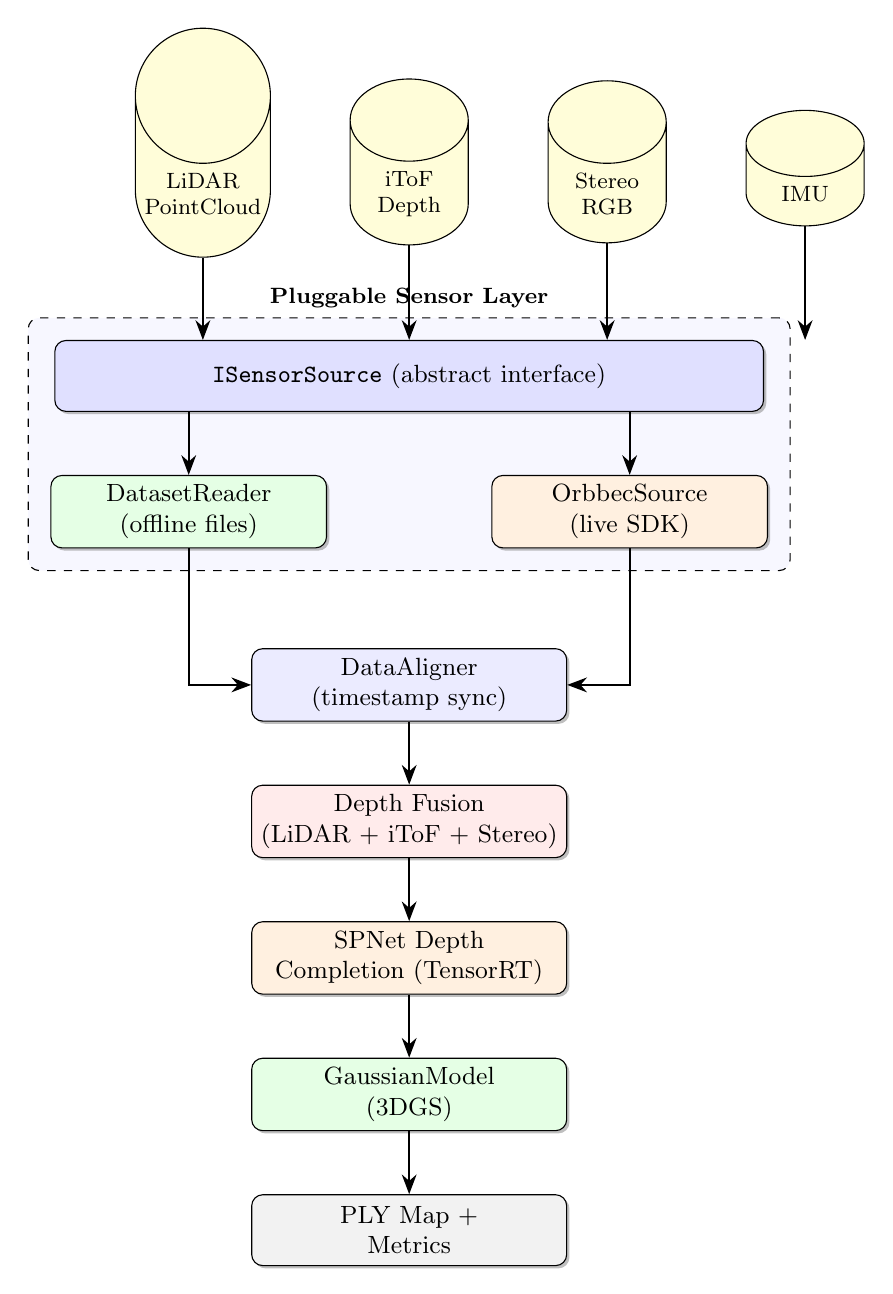
\begin{tikzpicture}[node distance=0.8cm and 1.0cm]

% ---- Row 1: Sensor sources ----
\node[sensor] (lidar)  {LiDAR\\PointCloud};
\node[sensor, right=of lidar] (itof)   {iToF\\Depth};
\node[sensor, right=of itof]  (stereo) {Stereo\\RGB};
\node[sensor, right=of stereo] (imu)   {IMU};

% ---- Row 2: ISensorSource interface ----
\node[block, below=1.2cm of itof, minimum width=9cm, fill=blue!12]
  (iface) {\texttt{ISensorSource} (abstract interface)};

% ---- Row 3: Concrete implementations (side by side) ----
\node[blockgreen, below=0.8cm of iface, xshift=-2.8cm, minimum width=3.5cm]
  (reader) {DatasetReader\\(offline files)};
\node[blockorange, below=0.8cm of iface, xshift=2.8cm, minimum width=3.5cm]
  (orbbec) {OrbbecSource\\(live SDK)};

% ---- Row 4: Data aligner ----
\node[block, below=of iface, yshift=-2.2cm, minimum width=4cm]
  (aligner) {DataAligner\\(timestamp sync)};

% ---- Row 5: Depth fusion ----
\node[blockred, below=of aligner, minimum width=4cm]
  (fusion) {Depth Fusion\\(LiDAR + iToF + Stereo)};

% ---- Row 6: Depth completion ----
\node[blockorange, below=of fusion, minimum width=4cm]
  (completer) {SPNet Depth\\Completion (TensorRT)};

% ---- Row 7: Gaussian model ----
\node[blockgreen, below=of completer, minimum width=4cm]
  (gaussian) {GaussianModel\\(3DGS)};

% ---- Row 8: Output ----
\node[block, below=of gaussian, minimum width=4cm, fill=gray!10]
  (output) {PLY Map +\\Metrics};

% ---- Arrows: sensors → interface ----
\draw[arrow] (lidar.south) -- (iface.north -| lidar.south);
\draw[arrow] (itof.south)  -- (iface.north -| itof.south);
\draw[arrow] (stereo.south)-- (iface.north -| stereo.south);
\draw[arrow] (imu.south)   -- (iface.north -| imu.south);

% ---- Arrows: interface → implementations ----
\draw[arrow] (iface.south -| reader.north) -- (reader.north);
\draw[arrow] (iface.south -| orbbec.north) -- (orbbec.north);

% ---- Arrows: implementations → aligner ----
\draw[arrow] (reader.south) |- (aligner.west);
\draw[arrow] (orbbec.south) |- (aligner.east);

% ---- Main pipeline arrows ----
\draw[arrow] (aligner) -- (fusion);
\draw[arrow] (fusion)  -- (completer);
\draw[arrow] (completer) -- (gaussian);
\draw[arrow] (gaussian) -- (output);

% ---- Group: Pluggable layer ----
\begin{scope}[on background layer]
  \node[group=Pluggable Sensor Layer, fit=(iface)(reader)(orbbec),
        fill=blue!3] (pluggable) {};
\end{scope}

\end{tikzpicture}
\caption{Overview of the \winlic{} processing pipeline. Multi-modal sensor
data enters through the pluggable \texttt{ISensorSource} abstraction, is
synchronized by the DataAligner, fused into a dense depth map, completed by
the SPNet TensorRT engine, and fed into the 3D Gaussian Splatting model for
reconstruction.}
\label{fig:pipeline}
\end{figure*}

The system comprises six stages:

\begin{enumerate}
    \item \textbf{Sensor Input.} Multi-modal data enters through an
    \texttt{ISensorSource} implementation---either a
    \texttt{DatasetReader} for offline files or an \texttt{OrbbecSource}
    for live camera streams.

    \item \textbf{Data Alignment.} The \texttt{DataAligner} synchronizes
    frames across modalities by timestamp, producing a single
    \texttt{AlignedFrame} struct containing the RGB image, LiDAR point
    cloud, depth maps from each source, IMU data, and camera pose.

    \item \textbf{Depth Fusion.} The \texttt{DepthFusion} module combines
    sparse LiDAR depth, dense iToF depth, and stereo SGM depth into a
    single confidence-weighted depth map (Section~\ref{sec:sensor_fusion}).

    \item \textbf{Depth Completion.} The fused depth map is completed by
    the SPNet TensorRT engine, which fills holes using RGB guidance.

    \item \textbf{Gaussian Reconstruction.} The completed depth map and
    fused point cloud are fed into the \texttt{GaussianModel}, which
    initializes, extends, and optimizes the 3D Gaussian map
    (Section~\ref{sec:gaussian_reconstruction}).

    \item \textbf{Output.} The final Gaussian map is exported as a PLY
    file, along with rendered images, depth visualizations, and quality
    metrics (PSNR, SSIM, LPIPS).
\end{enumerate}

\subsection{Data Structures}

The original \gaussianlic{} used ROS message types (\texttt{sensor\_msgs::Image},
\texttt{sensor\_msgs::PointCloud2}, \texttt{geometry\_msgs::PoseStamped})
as the inter-module data carriers. In \winlic, these are replaced by
ROS-free structs:

\begin{itemize}
    \item \texttt{PointXYZRGB}: A 3D point with 8-bit colour
    ($x, y, z, r, g, b$).
    \item \texttt{CameraPose}: Timestamped pose as an Eigen quaternion
    and translation vector.
    \item \texttt{ImuMeasurement}: Timestamped accelerometer and gyroscope
    readings.
    \item \texttt{AlignedFrame}: A self-contained frame containing the
    RGB image (\texttt{cv::Mat}), multiple depth maps, point cloud,
    pose, and metadata.
\end{itemize}

These structs use only OpenCV (\texttt{cv::Mat}) and Eigen
(\texttt{Eigen::Quaterniond}, \texttt{Eigen::Vector3d}) types, which are
fully portable across Windows and Linux.

\subsection{Build System}

The original system used \texttt{catkin} (ROS build system) with
\texttt{find\_package(catkin REQUIRED COMPONENTS roscpp rospy ...)}.
\winlic{} replaces this with a pure CMake build that links against
OpenCV, LibTorch (PyTorch C++ API), TensorRT, yaml-cpp, and CUDA.
The build is configured via CMake cache variables and supports both
MSVC (Windows) and GCC (Linux) out of the box.

% ===========================================================================
% Section: Multi-Modal Sensor Fusion
% ===========================================================================
\section{Multi-Modal Sensor Fusion}
\label{sec:sensor_fusion}

This section describes the two key components of the sensor fusion layer:
the pluggable \texttt{ISensorSource} interface and the multi-modal depth
fusion module.

\subsection{Pluggable Sensor Source Interface}
\label{subsec:sensor_interface}

The \texttt{ISensorSource} abstract interface (Figure~\ref{fig:sensor_architecture})
is the cornerstone of the framework's extensibility.

% ===========================================================================
% Figure: Sensor architecture — pluggable SDK interface
% Shows ISensorSource as an abstract interface with two concrete implementations.
% ===========================================================================
\begin{figure*}[t]
\centering
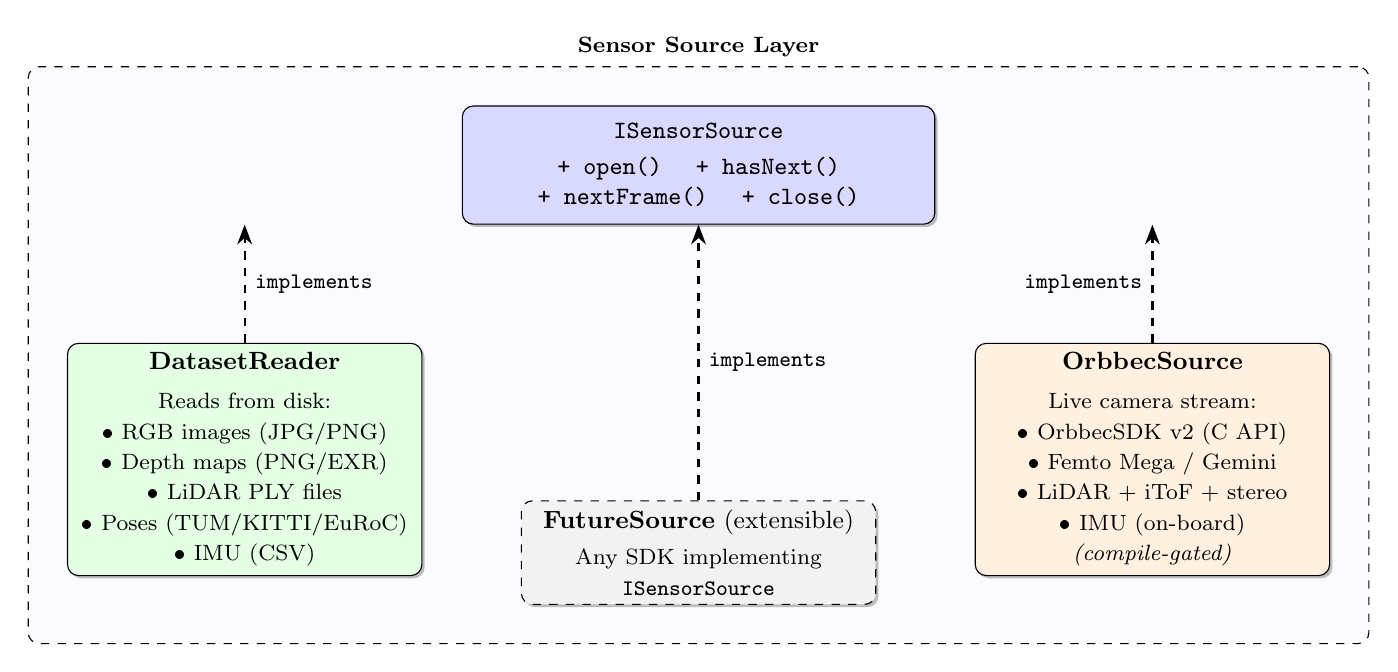
\begin{tikzpicture}[node distance=1.2cm]

% ---- Abstract interface (top) ----
\node[block, minimum width=6cm, minimum height=1.5cm, fill=blue!15]
  (iface) {\textbf{\texttt{ISensorSource}}\\[2pt]
           \texttt{+ open()} \quad \texttt{+ hasNext()}\\
           \texttt{+ nextFrame()} \quad \texttt{+ close()}};

% ---- Concrete implementations (bottom) ----
\node[blockgreen, below left=1.5cm and 0.5cm of iface, minimum width=4.5cm,
      minimum height=2.2cm]
  (reader) {\textbf{DatasetReader}\\[3pt]
            \footnotesize Reads from disk:\\
            \footnotesize • RGB images (JPG/PNG)\\
            \footnotesize • Depth maps (PNG/EXR)\\
            \footnotesize • LiDAR PLY files\\
            \footnotesize • Poses (TUM/KITTI/EuRoC)\\
            \footnotesize • IMU (CSV)};

\node[blockorange, below right=1.5cm and 0.5cm of iface, minimum width=4.5cm,
      minimum height=2.2cm]
  (orbbec) {\textbf{OrbbecSource}\\[3pt]
            \footnotesize Live camera stream:\\
            \footnotesize • OrbbecSDK v2 (C API)\\
            \footnotesize • Femto Mega / Gemini\\
            \footnotesize • LiDAR + iToF + stereo\\
            \footnotesize • IMU (on-board)\\
            \footnotesize \emph{(compile-gated)}};

% ---- Future extension ----
\node[block, below=3.5cm of iface, minimum width=4.5cm, fill=gray!10, dashed]
  (future) {\textbf{FutureSource} (extensible)\\[2pt]
            \footnotesize Any SDK implementing\\
            \footnotesize \texttt{ISensorSource}};

% ---- Inheritance arrows ----
\draw[dasharrow] (reader.north) -- (iface.south -| reader.north)
  node[midway, right, font=\footnotesize] {\texttt{implements}};
\draw[dasharrow] (orbbec.north) -- (iface.south -| orbbec.north)
  node[midway, left, font=\footnotesize] {\texttt{implements}};
\draw[dasharrow] (future.north) -- (iface.south)
  node[midway, right, font=\footnotesize] {\texttt{implements}};

% ---- Group ----
\begin{scope}[on background layer]
  \node[group=Sensor Source Layer, fit=(iface)(reader)(orbbec)(future),
        inner sep=14pt, fill=blue!2] {};
\end{scope}

\end{tikzpicture}
\caption{The \texttt{ISensorSource} abstract interface and its concrete
implementations. The \texttt{DatasetReader} handles offline file-based data,
while the \texttt{OrbbecSource} wraps the Orbbec SDK for live camera input.
The interface is designed for extensibility: any future sensor SDK can be
integrated by implementing four virtual methods.}
\label{fig:sensor_architecture}
\end{figure*}


It defines four virtual methods:

\begin{itemize}
    \item \texttt{open(config)}: Initialise the source from a YAML
    configuration node. For offline readers, this opens files and scans
    directories; for live cameras, this connects to the device and starts
    streaming.

    \item \texttt{hasNext()}: Poll whether more frames are available.
    For offline readers, this checks the frame index against the total
    count; for live cameras, this returns \texttt{true} until the stream
    is stopped.

    \item \texttt{nextFrame()}: Retrieve the next \texttt{AlignedFrame}.
    For offline readers, this loads the next set of files from disk;
    for live cameras, this blocks until the next frame set arrives.

    \item \texttt{close()}: Release resources.
\end{itemize}

\subsubsection{DatasetReader}

The \texttt{DatasetReader} is the primary sensor source for offline
processing. It reads from a structured directory layout:

\begin{verbatim}
base_path/
  images/         RGB frames (000000.jpg, ...)
  depth/          Depth maps (000000.png [16-bit mm] or .exr)
  pointclouds/    LiDAR PLY files (000000.ply, ...)
  trajectory.txt  Camera poses (TUM/KITTI/EuRoC format)
  imu.csv         IMU data (optional)
\end{verbatim}

Three pose formats are supported:
\begin{itemize}
    \item \textbf{TUM}: \texttt{timestamp tx ty tz qx qy qz qw}
    \item \textbf{KITTI}: 3$\times$4 row-major rigid transform matrix
    ($R | \mathbf{t}$), no timestamp
    \item \textbf{EuRoC}: CSV with nanosecond timestamps
    (\texttt{timestamp\_ns, px, py, pz, qw, qx, qy, qz})
\end{itemize}

Depth maps are loaded as 32-bit float images in metric units. PNG files
store depth in millimetres (16-bit unsigned) and are automatically
converted; EXR files store metric depth directly.

Point clouds are read via a minimal PLY parser that supports both ASCII
and binary little-endian formats, handling \texttt{float32} XYZ coordinates
and \texttt{uchar} RGB colour.

\subsubsection{OrbbecSource}

The \texttt{OrbbecSource} wraps the OrbbecSDK v2 C API for live data
acquisition from Orbbec 3D cameras (Femto Mega, Gemini 2). It enables
three streams---colour (RGB), depth (iToF), and IR/LiDAR---and returns
\texttt{AlignedFrame} objects with the same structure as the offline
reader.

This implementation is \emph{compile-gated}: when the
\texttt{USE\_ORBBEC\_SDK} preprocessor macro is not defined, a stub
implementation is compiled that prints a helpful error message and
returns \texttt{false} from \texttt{open()}. This ensures the framework
compiles cleanly without the SDK, and users can enable live camera
support by installing the SDK and passing
\texttt{-DUSE\_ORBBEC\_SDK=ON} to CMake.

\subsection{Multi-Modal Depth Fusion}
\label{subsec:depth_fusion}

The depth fusion module (Figure~\ref{fig:depth_fusion}) combines three
depth sources into a single high-quality depth map.

% ===========================================================================
% Figure: Multi-modal depth fusion data flow
% LiDAR sparse + iToF dense + stereo SGM → confidence weighting → SPNet
% ===========================================================================
\begin{figure*}[t]
\centering
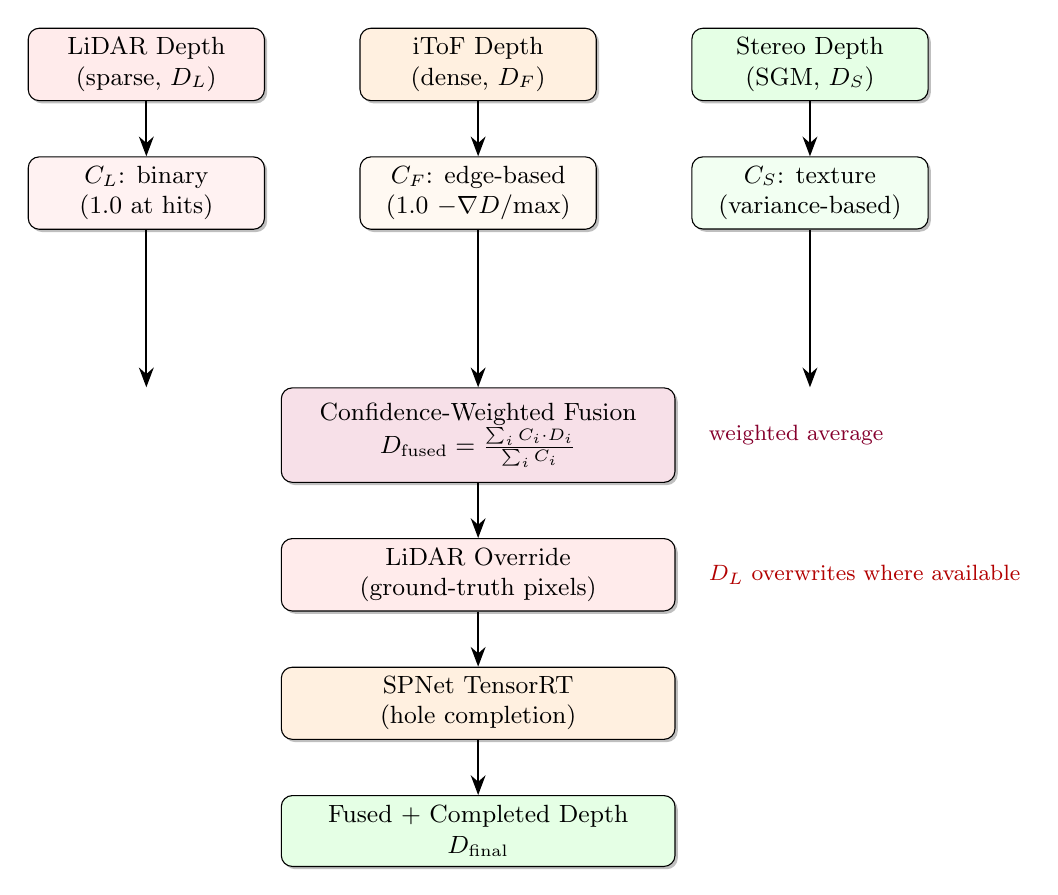
\begin{tikzpicture}[node distance=0.7cm and 1.2cm]

% ---- Row 1: Three depth sources ----
\node[blockred, minimum width=3cm] (lidar_d) {LiDAR Depth\\(sparse, $D_L$)};
\node[blockorange, right=of lidar_d, minimum width=3cm] (itof_d)
  {iToF Depth\\(dense, $D_F$)};
\node[blockgreen, right=of itof_d, minimum width=3cm] (stereo_d)
  {Stereo Depth\\(SGM, $D_S$)};

% ---- Row 2: Confidence maps ----
\node[block, below=of lidar_d, minimum width=3cm, fill=red!5]
  (conf_l) {$C_L$: binary\\(1.0 at hits)};
\node[block, below=of itof_d, minimum width=3cm, fill=orange!5]
  (conf_f) {$C_F$: edge-based\\(1.0 $- \nabla D$/max)};
\node[block, below=of stereo_d, minimum width=3cm, fill=green!5]
  (conf_s) {$C_S$: texture\\(variance-based)};

% ---- Row 3: Fusion node ----
\node[block, below=2.0cm of conf_f, minimum width=5cm, minimum height=1.2cm,
      fill=purple!12]
  (fuse) {Confidence-Weighted Fusion\\
          $D_{\text{fused}} = \frac{\sum_i C_i \cdot D_i}{\sum_i C_i}$};

% ---- Row 4: LiDAR override ----
\node[blockred, below=0.7cm of fuse, minimum width=5cm]
  (override) {LiDAR Override\\(ground-truth pixels)};

% ---- Row 5: SPNet completion ----
\node[blockorange, below=0.7cm of override, minimum width=5cm]
  (spnet) {SPNet TensorRT\\(hole completion)};

% ---- Row 6: Final depth ----
\node[blockgreen, below=0.7cm of spnet, minimum width=5cm]
  (final) {Fused + Completed Depth\\$D_{\text{final}}$};

% ---- Arrows: sources → confidence ----
\draw[arrow] (lidar_d) -- (conf_l);
\draw[arrow] (itof_d)  -- (conf_f);
\draw[arrow] (stereo_d)-- (conf_s);

% ---- Arrows: confidence → fusion ----
\draw[arrow] (conf_l.south) -- (fuse.north -| conf_l.south);
\draw[arrow] (conf_f.south) -- (fuse.north);
\draw[arrow] (conf_s.south) -- (fuse.north -| conf_s.south);

% ---- Main flow ----
\draw[arrow] (fuse) -- (override);
\draw[arrow] (override) -- (spnet);
\draw[arrow] (spnet) -- (final);

% ---- Annotations ----
\node[font=\footnotesize, right=0.3cm of fuse, text=purple!70!black]
  {weighted average};
\node[font=\footnotesize, right=0.3cm of override, text=red!70!black]
  {$D_L$ overwrites where available};

\end{tikzpicture}
\caption{Multi-modal depth fusion pipeline. Three depth sources---sparse
LiDAR, dense iToF, and stereo SGM---are each assigned a confidence map.
A weighted average produces the fused depth, after which LiDAR pixels
overwrite the fused result as ground truth. The SPNet TensorRT engine
completes remaining holes.}
\label{fig:depth_fusion}
\end{figure*}


Each source has
complementary characteristics:

\begin{table}[h]
\centering
\caption{Depth source characteristics.}
\label{tab:depth_sources}
\begin{tabular}{lccc}
\toprule
Source & Density & Accuracy & Limitation \\
\midrule
LiDAR  & Sparse ($\sim$5\% pixels) & High ($\pm$2\,cm) & Limited spatial coverage \\
iToF   & Dense (100\%) & Medium ($\pm$5\,cm) & Noise at discontinuities \\
Stereo & Dense (100\%) & Medium ($\pm$10\,cm) & Fails in textureless areas \\
\bottomrule
\end{tabular}
\end{table}

\subsubsection{LiDAR Depth Projection}

LiDAR points in the world frame are projected into the camera image to
produce a sparse depth map. Given a point $\mathbf{p}_w$ and camera pose
$(R_{wc}, \mathbf{t}_{wc})$:

\begin{align}
    \mathbf{p}_c &= R_{cw} \, \mathbf{p}_w + \mathbf{t}_{cw} \\
    u &= f_x \, p_{c,x} / p_{c,z} + c_x \\
    v &= f_y \, p_{c,y} / p_{c,z} + c_y
\end{align}

A Z-buffer ensures that the nearest depth is retained when multiple
points project to the same pixel.

\subsubsection{Stereo Depth via SGM}

When stereo image pairs are available, depth is computed via OpenCV's
\texttt{StereoSGBM} (Semi-Global Block Matching). The disparity map $d(u,v)$
is converted to metric depth:

\begin{equation}
    Z(u,v) = \frac{b \cdot f_x}{d(u,v)}
\end{equation}

where $b$ is the stereo baseline and $f_x$ is the horizontal focal length.

\subsubsection{Confidence-Weighted Fusion}

Each depth source is assigned a per-pixel confidence weight $C_i(u,v)$:

\begin{itemize}
    \item \textbf{LiDAR} ($C_L$): Binary---1.0 at pixels with LiDAR hits,
    0 elsewhere. LiDAR depth is treated as ground truth.

    \item \textbf{iToF} ($C_F$): Edge-based confidence, reduced at depth
    discontinuities:
    $C_F = 1 - \|\nabla D_F\| / \max\|\nabla D_F\|$.

    \item \textbf{Stereo} ($C_S$): Texture-based confidence, proportional
    to local depth variance (a proxy for scene texture).
\end{itemize}

The fused depth is computed as a weighted average:
\begin{equation}
    D_{\text{fused}}(u,v) = \frac{\sum_{i \in \{L, F, S\}} C_i(u,v) \cdot D_i(u,v)}
                                  {\sum_{i \in \{L, F, S\}} C_i(u,v)}
\end{equation}

After fusion, LiDAR pixels overwrite the fused depth as ground truth:
$D_{\text{fused}}(u,v) \leftarrow D_L(u,v)$ wherever $D_L(u,v) > 0$.

\subsection{Timestamp-Based Data Alignment}

Figure~\ref{fig:data_alignment} illustrates the timestamp-based alignment
strategy.

% ===========================================================================
% Figure: Timestamp-based multi-modal data alignment
% Timeline showing synchronization across 4 modalities.
% ===========================================================================
\begin{figure*}[t]
\centering
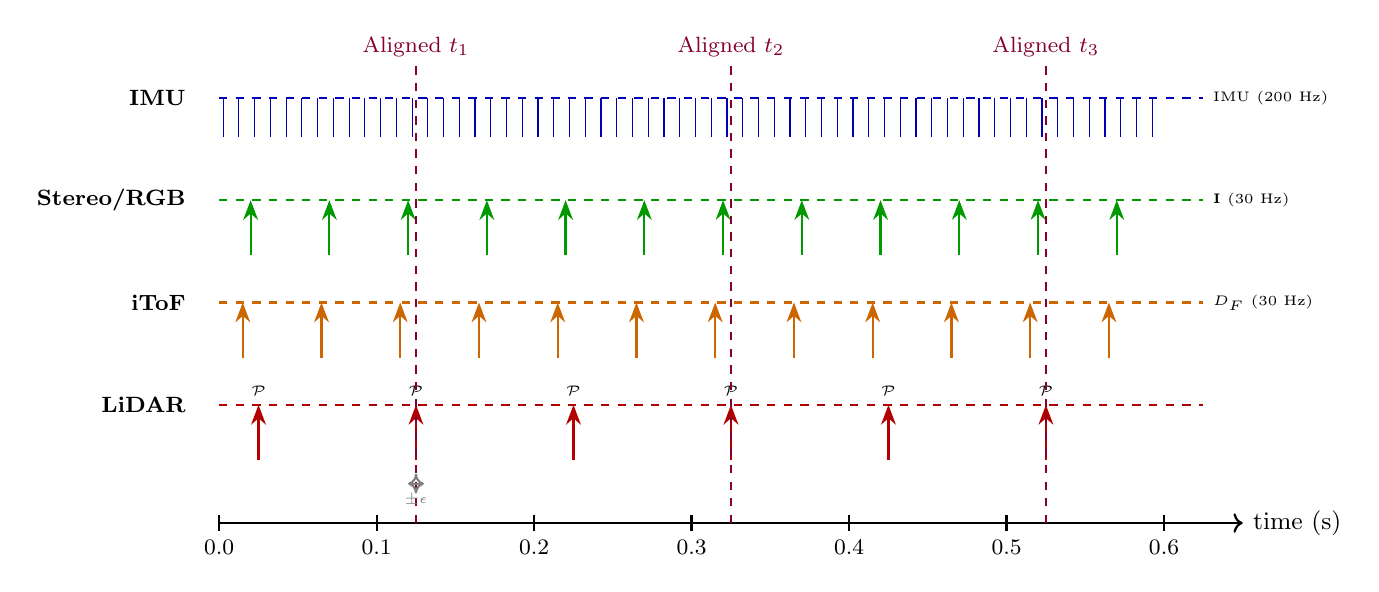
\begin{tikzpicture}[node distance=0.5cm, font=\small]

% ---- Timeline axis ----
\draw[->, thick] (0,0) -- (13,0) node[right] {time (s)};
\foreach \x/\label in {0/0.0, 2/0.1, 4/0.2, 6/0.3, 8/0.4, 10/0.5, 12/0.6}
{
  \draw[thick] (\x, -0.1) -- (\x, 0.1);
  \node[below, font=\footnotesize] at (\x, -0.1) {\label};
}

% ---- LiDAR row ----
\node[left, font=\footnotesize\bfseries] at (-0.3, 1.5) {LiDAR};
\foreach \x in {0.5, 2.5, 4.5, 6.5, 8.5, 10.5}
{
  \draw[arrow, red!70!black] (\x, 0.8) -- (\x, 1.5);
  \node[font=\tiny, above] at (\x, 1.5) {$\PointCloud$};
}
\draw[red!70!black, thick, dashed] (0, 1.5) -- (12.5, 1.5);

% ---- iToF row ----
\node[left, font=\footnotesize\bfseries] at (-0.3, 2.8) {iToF};
\foreach \x in {0.3, 1.3, 2.3, 3.3, 4.3, 5.3, 6.3, 7.3, 8.3, 9.3, 10.3, 11.3}
{
  \draw[arrow, orange!80!black] (\x, 2.1) -- (\x, 2.8);
}
\draw[orange!80!black, thick, dashed] (0, 2.8) -- (12.5, 2.8);
\node[font=\tiny, right] at (12.5, 2.8) {$D_F$ (30 Hz)};

% ---- Stereo/RGB row ----
\node[left, font=\footnotesize\bfseries] at (-0.3, 4.1) {Stereo/RGB};
\foreach \x in {0.4, 1.4, 2.4, 3.4, 4.4, 5.4, 6.4, 7.4, 8.4, 9.4, 10.4, 11.4}
{
  \draw[arrow, green!60!black] (\x, 3.4) -- (\x, 4.1);
}
\draw[green!60!black, thick, dashed] (0, 4.1) -- (12.5, 4.1);
\node[font=\tiny, right] at (12.5, 4.1) {$\Image$ (30 Hz)};

% ---- IMU row ----
\node[left, font=\footnotesize\bfseries] at (-0.3, 5.4) {IMU};
\foreach \x in {0.05, 0.25, 0.45, 0.65, 0.85, 1.05, 1.25, 1.45, 1.65, 1.85,
                2.05, 2.25, 2.45, 2.65, 2.85, 3.05, 3.25, 3.45, 3.65, 3.85,
                4.05, 4.25, 4.45, 4.65, 4.85, 5.05, 5.25, 5.45, 5.65, 5.85,
                6.05, 6.25, 6.45, 6.65, 6.85, 7.05, 7.25, 7.45, 7.65, 7.85,
                8.05, 8.25, 8.45, 8.65, 8.85, 9.05, 9.25, 9.45, 9.65, 9.85,
                10.05, 10.25, 10.45, 10.65, 10.85, 11.05, 11.25, 11.45, 11.65, 11.85}
{
  \draw[blue!70!black] (\x, 4.9) -- (\x, 5.4);
}
\draw[blue!70!black, thick, dashed] (0, 5.4) -- (12.5, 5.4);
\node[font=\tiny, right] at (12.5, 5.4) {IMU (200 Hz)};

% ---- Aligned frame markers ----
\foreach \x/\label in {2.5/$t_1$, 6.5/$t_2$, 10.5/$t_3$}
{
  \draw[thick, purple!70!black, dashed] (\x, 0) -- (\x, 5.8);
  \node[font=\footnotesize, above, purple!70!black] at (\x, 5.8) {Aligned \label};
}

% ---- Tolerance band ----
\draw[<->, thick, gray] (2.4, 0.5) -- (2.6, 0.5)
  node[midway, below, font=\tiny] {$\pm\epsilon$};

\end{tikzpicture}
\caption{Timestamp-based multi-modal data alignment. The LiDAR stream
(10--20\,Hz) defines the reference timestamps. iToF, stereo, and IMU data
are matched within a tolerance $\epsilon = 10$\,ms. Dashed vertical lines
mark aligned frame instances $t_1, t_2, t_3$ where all modalities are
synchronized.}
\label{fig:data_alignment}
\end{figure*}


The LiDAR stream (10--20\,Hz) defines the reference timestamps,
and other modalities are matched within a tolerance
$\epsilon = 10$\,ms. This mirrors the alignment logic in the original
\gaussianlic{} system, where ROS message timestamps were used for
queue-based synchronization.

In the offline \texttt{DatasetReader}, alignment is implicit because all
modalities share the same frame numbering. The \texttt{DataAligner}
class provides an explicit alignment utility for live streaming scenarios
where modalities arrive at different rates.

% ===========================================================================
% Section: Gaussian Reconstruction
% ===========================================================================
\section{Gaussian Splatting Reconstruction}
\label{sec:gaussian_reconstruction}

The reconstruction pipeline preserves the core algorithm of
\gaussianlic~\cite{lang2026_gaussianlic2} while replacing the ROS-based
data ingestion with the offline sensor source layer. This section
describes the four stages: initialization, frame addition, map extension,
and map optimization.

\subsection{Gaussian Initialization}
\label{subsec:init}

The Gaussian map is initialized from the first keyframe's fused point
cloud (Figure~\ref{fig:gaussian_init}).

% ===========================================================================
% Figure: Gaussian initialization from fused point cloud
% Fused point cloud → SH colour → scale estimation → 3DGS parameters
% ===========================================================================
\begin{figure*}[t]
\centering
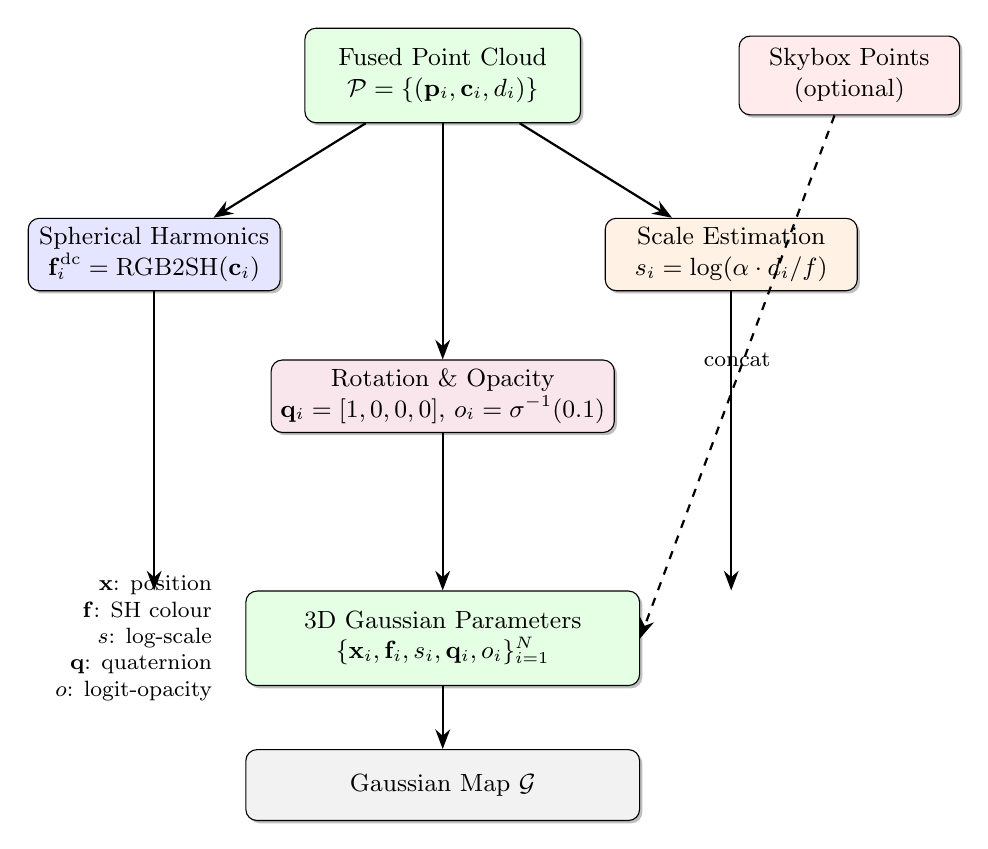
\begin{tikzpicture}[node distance=0.8cm and 1.0cm]

% ---- Input: Fused point cloud ----
\node[blockgreen, minimum width=3.5cm, minimum height=1.2cm]
  (cloud) {Fused Point Cloud\\$\PointCloud = \{(\mathbf{p}_i, \mathbf{c}_i, d_i)\}$};

% ---- Branch 1: SH colour ----
\node[block, below left=1.2cm and 0.3cm of cloud, minimum width=3.2cm, fill=blue!10]
  (sh) {Spherical Harmonics\\$\mathbf{f}_i^{\text{dc}} = \mathrm{RGB2SH}(\mathbf{c}_i)$};

% ---- Branch 2: Scale estimation ----
\node[block, below right=1.2cm and 0.3cm of cloud, minimum width=3.2cm, fill=orange!10]
  (scale) {Scale Estimation\\$s_i = \log\!\left(\alpha \cdot d_i / f\right)$};

% ---- Branch 3: Rotation & opacity ----
\node[block, below=3.0cm of cloud, minimum width=3.2cm, fill=purple!10]
  (rot) {Rotation \& Opacity\\$\mathbf{q}_i = [1,0,0,0]$, $o_i = \sigma^{-1}(0.1)$};

% ---- Merge: 3DGS parameters ----
\node[blockgreen, below=2.0cm of rot, minimum width=5cm, minimum height=1.2cm]
  (params) {3D Gaussian Parameters\\
            $\{\mathbf{x}_i, \mathbf{f}_i, s_i, \mathbf{q}_i, o_i\}_{i=1}^{N}$};

% ---- Output: Gaussian map ----
\node[block, below=of params, minimum width=5cm, fill=gray!10]
  (map) {Gaussian Map $\GaussianMap$};

% ---- Arrows ----
\draw[arrow] (cloud) -- (sh);
\draw[arrow] (cloud) -- (scale);
\draw[arrow] (cloud) -- (rot);
\draw[arrow] (sh)    -- (params.north -| sh.south);
\draw[arrow] (scale) -- (params.north -| scale.south);
\draw[arrow] (rot)   -- (params);
\draw[arrow] (params) -- (map);

% ---- Skybox (optional, side branch) ----
\node[blockred, right=2.0cm of cloud, minimum width=2.8cm, minimum height=1.0cm]
  (sky) {Skybox Points\\(optional)};
\draw[dasharrow] (sky) -- (params.east)
  node[midway, above, font=\footnotesize] {concat};

% ---- Annotation ----
\node[font=\footnotesize, left=0.3cm of params, align=right]
  {$\mathbf{x}$: position\\$\mathbf{f}$: SH colour\\$s$: log-scale\\$\mathbf{q}$: quaternion\\$o$: logit-opacity};

\end{tikzpicture}
\caption{Gaussian initialization from the fused point cloud. Each 3D point
$\mathbf{p}_i$ with colour $\mathbf{c}_i$ and camera-frame depth $d_i$ is
converted to a Gaussian primitive with position, SH colour coefficients,
log-scale (derived from depth and focal length), identity rotation, and
initial opacity. Optional skybox points are appended for open-environment
scenes.}
\label{fig:gaussian_init}
\end{figure*}


For each 3D point
$\mathbf{p}_i$ with colour $\mathbf{c}_i$ and camera-frame depth $d_i$,
a Gaussian primitive is created with the following parameters:

\begin{itemize}
    \item \textbf{Position} $\mathbf{x}_i = \mathbf{p}_i$ (world frame).
    \item \textbf{Colour (SH)}: The RGB colour is converted to zeroth-order
    spherical harmonics:
    $\mathbf{f}_i^{\text{dc}} = (\mathbf{c}_i - 0.5) / C_0$,
    where $C_0 = 0.28209$.
    \item \textbf{Scale}: $s_i = \log(\alpha \cdot d_i / f)$, where
    $\alpha$ is a scaling factor and $f$ is the average focal length.
    The log-parameterization ensures positivity after exponentiation.
    \item \textbf{Rotation}: Identity quaternion $[1, 0, 0, 0]$.
    \item \textbf{Opacity}: $\sigma^{-1}(0.1)$, the inverse sigmoid of 0.1.
\end{itemize}

For outdoor scenes, optional skybox points are added: $N_{\text{sky}}$
points uniformly distributed on a sphere of radius $10 \cdot R_{\text{sky}}$,
with a light-blue colour and higher initial opacity (0.7).

\subsection{Frame Addition and Depth Completion}

Each incoming aligned frame is added to the dataset. The RGB image is
converted from BGR (0--255) to RGB float (0--1). The fused depth map is
optionally completed by the SPNet TensorRT engine, which takes the RGB
image and sparse depth as input and produces a dense depth map.

After depth completion, the system selects patches where the completed
depth disagrees with the known LiDAR depth by less than 0.1\,m (mean
difference). In non-edge, positive-depth regions, additional 3D points
are back-projected from the completed depth at patch-level granularity,
enriching the point cloud with denser colour observations.

Keyframes are selected every $k$-th frame (default $k=5$). Keyframes are
added to the training set; non-keyframes to the test set for novel-view
evaluation.

\subsection{Map Extension}

When a new keyframe arrives and the map is already initialized, the
\texttt{extend} function adds new Gaussian primitives from the current
frame's point cloud. The process:

\begin{enumerate}
    \item Render the current viewpoint to obtain an alpha map
    (existing coverage).
    \item Project the new LiDAR points into the image plane and perform
    z-buffering to keep the nearest point per pixel.
    \item Filter out points that are: (a) outside the image bounds,
    (b) at non-positive depth, or (c) in already-opaque regions
    ($\alpha > 0.99$).
    \item Create Gaussian primitives for the surviving points with SH
    colour, log-scale from depth, identity rotation, and low initial
    opacity.
    \item Append to the existing Gaussian parameters via
    \texttt{densificationPostfix}, which also extends the optimizer state
    (Adam moments) for the new parameters.
\end{enumerate}

A memory safety cap (\texttt{max\_gaussians}) limits the total Gaussian
count on memory-constrained GPUs. When the budget is exceeded, new points
are randomly subsampled to fit the remaining budget.

\subsection{Map Optimization}

After each keyframe, the map is optimized by rendering a random subset of
training viewpoints and minimizing a photometric loss:

\begin{equation}
    \mathcal{L} = (1 - \lambda_{\text{dssim}}) \, \mathcal{L}_1
                + \lambda_{\text{dssim}} \, (1 - \text{SSIM})
                + \lambda_{\text{depth}} \, \mathcal{L}_{\text{depth}}
\end{equation}

where $\mathcal{L}_1$ is the L1 error between rendered and ground-truth
images, SSIM is computed via a fused CUDA kernel for efficiency, and
$\mathcal{L}_{\text{depth}}$ is the L1 error on depth where both rendered
and ground-truth depth are valid.

The optimizer is a custom \texttt{SparseGaussianAdam} that updates only
the Gaussians visible in the current rendered viewpoint, reducing
computational cost. The visibility mask is obtained from the rasterizer's
forward pass.

\subsection{Evaluation and Export}

After all frames are processed, the system evaluates visual quality on
both training and novel (test) viewpoints, computing PSNR, SSIM, and
LPIPS (using a pre-computed AlexNet-based LPIPS model loaded via TorchScript).

The final Gaussian map is exported as a binary PLY file with per-vertex
properties: position ($x, y, z$), SH DC coefficients, SH rest coefficients,
opacity, scale, and rotation. This format is compatible with standard
3DGS viewers such as the SIBR\_gaussianViewer and web-based renderers.

% ===========================================================================
% Section: Experiments (placeholder for future results)
% ===========================================================================
\section{Experimental Setup}
\label{sec:experiments}

\subsection{Implementation Details}

\winlic{} is implemented in C++17 with CUDA 11.7 and built using CMake 3.18+.
The framework depends on LibTorch 2.0 (PyTorch C++ API), OpenCV 4.7 (with
CUDA and opencv\_contrib), TensorRT 8.6 (for SPNet depth completion),
yaml-cpp 0.6, and Eigen 3.4. The build supports both MSVC 2022 (Windows)
and GCC 9+ (Linux) with no platform-specific preprocessor directives
beyond CUDA architecture selection.

The SPNet depth completion engine is pre-compiled as a TensorRT plan file
(\texttt{.engine}) for two resolutions: 480$\times$640 and 512$\times$640.
The LPIPS model is exported as a TorchScript module (\texttt{lpips\_alex.pt}).

\subsection{Datasets}

The framework is designed to process data from the following sources:

\begin{itemize}
    \item \textbf{FAST-LIVO2 datasets}: Pre-recorded LiDAR-visual-inertial
    sequences with poses from the FAST-LIVO2 odometry front-end. The
    trajectory is exported in TUM format for offline processing.

    \item \textbf{MCD (Multi-Camera Dataset)}: Outdoor urban sequences
    with LiDAR, camera, and IMU data.

    \item \textbf{R3LIVE datasets}: RGB-LiDAR fusion sequences for
    indoor and outdoor scenes.

    \item \textbf{Custom Orbbec captures}: Live data from Orbbec Femto
    Mega cameras (LiDAR + iToF + stereo + IMU), recorded via the
    \texttt{OrbbecSource} and exported for offline processing.
\end{itemize}

\subsection{Metrics}

Reconstruction quality is evaluated using standard metrics:

\begin{itemize}
    \item \textbf{PSNR} (Peak Signal-to-Noise Ratio): measures pixel-level
    fidelity of rendered images.
    \item \textbf{SSIM} (Structural Similarity Index): measures perceptual
    quality via luminance, contrast, and structure.
    \item \textbf{LPIPS} (Learned Perceptual Image Patch Similarity):
    measures perceptual distance using deep features from AlexNet.
\end{itemize}

Metrics are computed on both training viewpoints (keyframes used during
optimization) and novel viewpoints (intermediate frames not used for
training), providing a measure of generalization.

\subsection{Baseline Comparison}

The primary baseline is the original \gaussianlic{} system running on
Linux with ROS. Since \winlic{} preserves the Gaussian Splatting algorithm
verbatim, we expect identical reconstruction quality (PSNR, SSIM, LPIPS)
when processing the same data. Differences may arise from:

\begin{itemize}
    \item Floating-point determinism between MSVC and GCC.
    \item Depth completion quality when using fused depth (LiDAR + iToF + stereo)
    versus LiDAR-only depth.
    \item Frame alignment differences between ROS timestamp-based and
    file-index-based synchronization.
\end{itemize}

\subsection{Runtime Analysis}

The offline processing mode eliminates the real-time constraint, allowing
the system to process each frame at full speed without buffer overflow
concerns. Expected runtime on an NVIDIA RTX~4090:
\begin{itemize}
    \item Depth fusion: $\sim$5\,ms/frame
    \item SPNet completion: $\sim$10\,ms/frame
    \item Gaussian extension: $\sim$50\,ms/keyframe
    \item Gaussian optimization: $\sim$500\,ms/keyframe (100 iterations)
\end{itemize}

\subsection{Ablation Studies}

Planned ablation studies include:
\begin{itemize}
    \item Effect of depth fusion: LiDAR-only vs.\ LiDAR+iToF vs.\ LiDAR+iToF+stereo.
    \item Effect of keyframe interval: $k \in \{1, 3, 5, 10\}$.
    \item Effect of Gaussian memory cap on quality vs.\ memory usage.
    \item Effect of SH degree on rendering quality.
\end{itemize}

\begin{table}[h]
\centering
\caption{Default hyperparameters (preserved from \gaussianlic).}
\label{tab:hyperparams}
\begin{tabular}{lc}
\toprule
Parameter & Value \\
\midrule
Image resolution & $640 \times 512$ \\
SH degree & 3 \\
Keyframe interval $k$ & 5 \\
Position learning rate & $1.6 \times 10^{-4}$ \\
Feature learning rate & $5.0 \times 10^{-3}$ \\
Opacity learning rate & $5.0 \times 10^{-2}$ \\
Scaling learning rate & $5.0 \times 10^{-3}$ \\
Rotation learning rate & $1.0 \times 10^{-3}$ \\
$\lambda_{\text{dssim}}$ & 0.2 \\
$\lambda_{\text{depth}}$ & 0.005 \\
Optimization iterations & 100/keyframe \\
Max depth & 20\,m \\
\bottomrule
\end{tabular}
\end{table}

% ===========================================================================
% Section: Conclusion
% ===========================================================================
\section{Conclusion}
\label{sec:conclusion}

We have presented \winlic, a Windows-compatible offline multi-modal
Gaussian Splatting framework that eliminates the ROS dependency of prior
Gaussian SLAM systems. The framework makes three key contributions:

\begin{enumerate}
    \item A \textbf{pluggable sensor source interface} (\texttt{ISensorSource})
    that decouples the reconstruction pipeline from data acquisition,
    supporting both offline file-based datasets and live Orbbec camera
    streams through a uniform four-method interface. The design is
    extensible to future sensor SDKs without pipeline modification.

    \item A \textbf{multi-modal depth fusion} module that combines sparse
    LiDAR depth, dense iToF depth, and stereo SGM depth via
    confidence-weighted averaging, producing higher-quality depth maps
    than any single modality. The fused depth is further refined by the
    SPNet TensorRT completion engine.

    \item A \textbf{ROS-free, cross-platform build} that runs on both
    Windows (MSVC) and Linux (GCC) with pure CMake, preserving the core
    Gaussian Splatting algorithm of \gaussianlic{} without quality
    degradation.
\end{enumerate}

\subsection{Limitations and Future Work}

The current framework has several limitations that we plan to address:

\begin{itemize}
    \item \textbf{Pose dependency:} The system relies on pre-computed
    poses from an external SLAM front-end (e.g., FAST-LIVO2). Integrating
    a lightweight LIO frontend would enable fully self-contained
    processing, though at the cost of additional platform dependencies
    (PCL, IKFOM).

    \item \textbf{Orbbec SDK integration:} The current implementation
    provides a stub for the Orbbec SDK. Full integration with live
    streaming and on-device point-cloud generation requires testing
    with physical hardware.

    \item \textbf{GUI:} The current CLI interface is sufficient for
    batch processing but lacks interactive visualization. A Qt or
    Dear~ImGui-based GUI would improve usability for parameter tuning
    and real-time preview.

    \item \textbf{Large-scale scenes:} The in-memory Gaussian
    representation does not support out-of-core processing. For
    city-scale scenes, a submap-based tiling strategy (similar to
    Co-LIC2) would be needed.
\end{itemize}

\subsection{Reproducibility}

The complete source code, build instructions, and configuration files
are provided in the \texttt{win\_lic/} directory of the project repository.
The original ROS-based code in \texttt{src/} is preserved untouched,
allowing direct comparison between the two implementations.


\bibliographystyle{plain}
\bibliography{refs}

\end{document}
